% E: x^2/16+y^2/12=1; H: x^2-y^2/3=1.
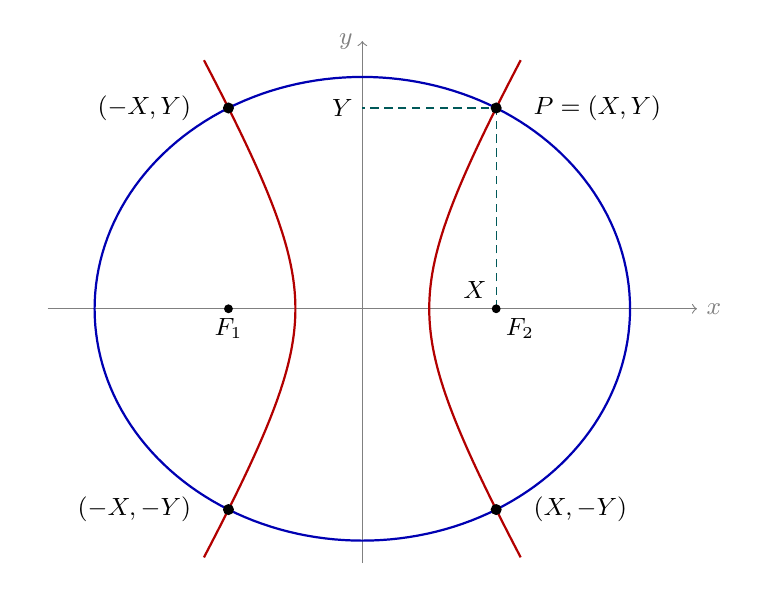
\begin{tikzpicture}[x=.85cm,y=.85cm,every node/.style={font=\small}]
\path[use as bounding box] (-5,-4.1) rectangle (5.8,4.2);
\draw[->,gray] (-4.7,0)--(5,0) node[right] {$x$};
\draw[->,gray] (0,-3.8)--(0,4) node[left] {$y$};
\draw[blue!70!black,thick,domain=0:360,samples=181,variable=\t] plot ({4*cos(\t)},{sqrt(12)*sin(\t)});
\foreach \sgn in {-1,1} \draw[red!70!black,thick,domain=-65:65,samples=121,variable=\t] plot ({\sgn/cos(\t)},{sqrt(3)*tan(\t)});
\draw[densely dashed,teal!70!black] (2,0)--(2,3)--(0,3);
\foreach \x in {-2,2} \foreach \y in {-3,3} \fill (\x,\y) circle(2pt);
\node[right,xshift=10pt] at (2,3) {$P=(X,Y)$};
\node[left,xshift=-10pt] at (-2,3) {$(-X,Y)$};
\node[left,xshift=-10pt] at (-2,-3) {$(-X,-Y)$};
\node[right,xshift=10pt] at (2,-3) {$(X,-Y)$};
\fill (-2,0) circle(1.6pt) node[below] {$F_1$};
\fill (2,0) circle(1.6pt) node[below right] {$F_2$};
\node[above left] at (2,0) {$X$}; \node[left] at (0,3) {$Y$};
\end{tikzpicture}
